\chapter{Liqo}

Due to the rapid adoption of containers as the development environment for applications, there is now a well-established trend towards using orchestration platforms to automate the lifecycle management of containerized applications. Among the various implementations of these platforms, Kubernetes has gained predominant traction, to the extent that multinational corporations with dedicated cloud departments (such as Google, Amazon, Microsoft, Alibaba...) have developed proprietary solutions based on it. Recently, a trend similar to the one observed with container adoption has emerged, in which there is a growing need for a system that can automate relationships between various clusters managed by these platforms, whether in the cloud or on-premise. Liqo is a project designed to address this necessity, described by its creators as "an open-source project that enables dynamic and seamless Kubernetes multi-cluster topologies, supporting heterogeneous on-premise, cloud, and edge infrastructures."

\section{Basic concepts}
The Liqo technology facilitates the creation of a unified virtual network across diverse clusters, enabling the execution of application pods on remote clusters as if they were local. This system is founded on four primary characteristics: network fabric, peering, offloading, storage fabric

\subsection{network fabric}
The network fabric is the subsystem of Liqo that seamlessly extends the Kubernetes networking model across multiple independent clusters, enabling pods on different clusters to communicate smoothly even when address NAT is applied.
The control plane of this subsystem resides in the network manager, instantiated as a pod responsible for managing network parameters. It handles tasks both during cluster peering and inter-cluster communications, as example featuring an interface used by the reflection logic for IP address translation.
Interconnecting two clusters involves deploying a secure VPN tunnel using WireGuard(CITA DOC? non di interesse), typically established at the end of the peering process based on negotiated parameters. This functionality is implemented by the Liqo gateway component, operating within the cluster as a privileged pod. It also manages routing tables and configures necessary NAT rules to resolve address conflicts. Although initialized within the cluster's network, this pod utilizes a separate network namespace and policy routing to avoid conflicts with Kubernetes' existing Container Network Interface (CNI) plugins.
Traffic from local nodes/pods directed to a remote cluster is routed through an overlay network, based on VXLAN, managed by a DaemonSet component. This component is responsible for routing entries and ensures proper handling of traffic across the VPN tunnels.

\subsection{Peering}
Standard peering is the process that establishes a unidirectional link between two different Kubernetes clusters, enabling the sharing of resources and services. Through this connection, the consumer cluster can initiate processes using resources provided by the provider cluster, but not vice versa. In this context, the consumer cluster initiates an outgoing peering towards the provider, which reciprocates with an incoming peering from the consumer. This linkage is not exclusive, supporting possible bidirectionality and the scenario where a cluster can act as a consumer for some peerings and as a provider for others.
The peering process unfolds through the following steps:
\begin{enumerate}
\item Authentication: Each cluster uses a pre-shared token to verify its identity, which has some permissions for Liqo-related resources and negotiations.
\item Parameter Negotiation: The two clusters exchange sets of parameters necessary for finalizing the peering, including network information such as their respective CIDRs or as the amount of resources shared by the provider. Some of these parameters can be modified directly or using dedicated plugins, for example is possible adjusting the available resources that the provider cluster shows to the consumer cluster.
\item Creation of the Virtual Node: Within the consumer cluster, a virtual node is created to represent the resources shared by the provider cluster. Processes instantiated using the provider cluster's resources appear to be located within this virtual node, maintaining transparency in the offloading process and adhering to standard Kubernetes practices without requiring API modifications.
\item Configuration of the Network Fabric: The two clusters configure their respective network fabrics and establish a secure VPN tunnel using the previously negotiated parameters (address remapping, endpoints, etc.).
\end{enumerate}
Each connection can be differentiated based on how Liqo's control plane traffic is managed: whether it passes through the VPN tunnel alongside pod traffic (in-band control plane peering) or uses traditional communication channels (out-of-band control plane peering). In the former case, it is required to expose only the Liqo VPN endpoint to the pod of the remote cluster. However, this setup requires control over both clusters to negotiate network parameters through Liqo CTL tool (CITA DOC?), resulting in a static peering configuration that requires manual intervention for updates. In the latter case, while to the remote pods must be expose not only the Liqo VPN endpoint but also the Kubernetes API and Liqo authentication service endpoints, it offers the flexibility to connect clusters across different domains using a pre-shared token and enables dynamic peering, so that an automatic renegotiation of parameters occurs in response to configuration changes. 

\begin{figure}[htb]\centering
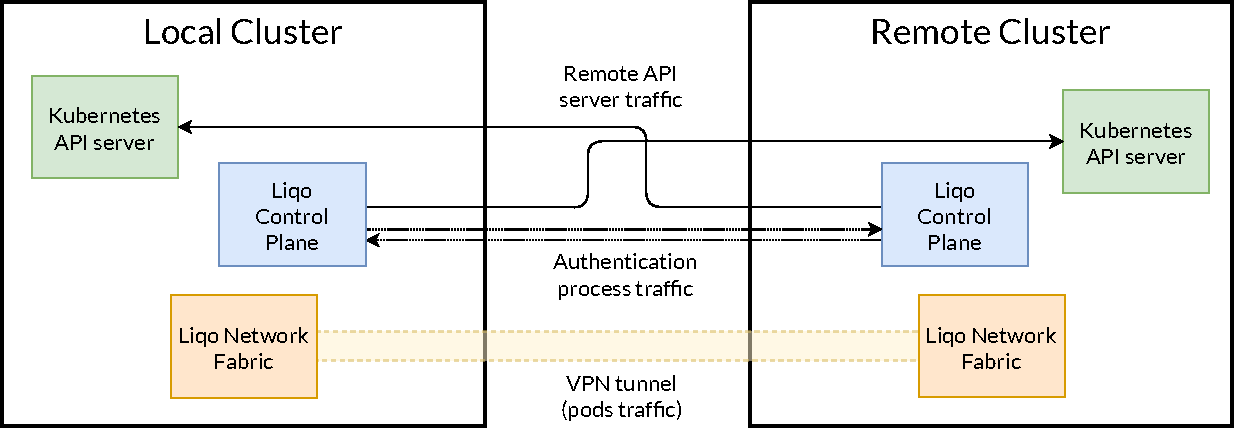
\includegraphics[scale=.5] {Pictures/out-of-band}
\caption{Out-of-band control plane peering (url)}\label{fig:figura}
\end{figure}

\subsection{offloading}
Offloading is the method enabling transparent extension of the local cluster into a remote cluster, allowing Kubernetes scheduler to seamlessly schedule workloads in the remote cluster when it's deemed optimal. The virtual node is managed by an extended version of the Virtual Kubelet project, which replaces the traditional kubelet if the node isn't physical. In the context of Liqo, it interacts with the Kubernetes API servers of both clusters to manage artifact propagation (pods, services, config maps) and reconcile state in case of changes on the negotiated configurations. It also performs configurable periodic health checks to assess reachability of the remote API server, marking the node as unready in case of repeated failures and triggering standard Kubernetes evacuation strategies. An instance of the virtual kubelet is created for each remote cluster to ensure isolation and segregation of authentication tokens.
The offloading process comprises three stages:
\begin{enumerate}
\item Namespace Extension: The local cluster's namespace is extended into the remote cluster by creating a gemini counterpart namespace, which will host both offloaded pods and resources required for pod reflection.
\item Resource Reflection: Selected arctifacts from the control plane are reflected in remote clusters to ensure the operational functionality of the pods. Supported resources for reflection include service exposure (Ingress, Services, EndpointSlices), persistent storage (PersistentVolumeClaims, PersistentVolumes), and configuration data (ConfigMaps, Secrets).
\item Pod Offloading: After the scheduler schedules a pod on the virtual node, the corresponding virtual kubelet creates a mirrored pod object in the remote cluster. This object is managed by the custom resource ShadowPod, serving as a representation of the pod to maintain service functionality even if connectivity with the remote cluster is lost (CITA https://webthesis.biblio.polito.it/secure/21145/1/tesi.pdf).
\end{enumerate}
Both stateless and stateful pods are supported, with the latter utilizing either the storage fabric or relying on an external volume provider.

\subsection{storage fabric}
The storage fabric is the Liqo subsystem responsible for managing the creation of remote volumes for stateful applications. Its operation revolves around delaying the binding of a volume to a pod until it has been scheduled to a node, ensuring volumes are always created where their associated pod is scheduled. Subsequent scheduling adheres to a data gravity principle, transparently rescheduling the pod to the node where the physical volume resides. These behaviors are implemented through Liqo's virtual storage class, utilizing reflection mechanisms when pods are scheduled on virtual nodes to create the mirrored PVCs in remote clusters. Alternatively, it relies on the real storage class when pods are scheduled on local physical nodes.

\section{Distributed DB interaction}
At present, Liqo does not fully support architectures of distributed database systems, primarily due to their reliance on internal headless services for direct pod-to-pod communication. These services return the IP address of the corresponding pod directly when queried, using their DNS entry, unlike regular services that route requests via kube-proxy. Liqo employs an address remapping mechanism to facilitate seamless communication between clusters; however, this approach results in incorrect IP resolutions for pods scheduled on remote clusters when queried by headless services.
To enable the use of these architectures, Liqo developers currently recommend (CITA ISSUE GITHUB) leveraging the peering process, which exposes the address ranges of the two clusters in two different ways:
\begin{enumerate}
\item Connecting a cluster to all others via peering while forcing a pod of the distributed system onto it: This approach ensures that the service in that cluster is aware of all real address ranges, allowing replication through the forced pod, which becomes a critical point.
\item Creating a full mesh of peering between various clusters: This ensures that each headless service knows the addresses of all others, and this is the solution adopted in this research
\end{enumerate}
Some distributed database architectures, such as those implemented by the Percona XtraDB Cluster Operator, may introduce additional complexity. After receiving the translated IP of a remote pod, they may encounter difficulties establishing a connection, primarily because their cluster logic operates with standard Kubernetes component independently of Liqo. This requires the implementation of distinct CIDRs across clusters, ensuring that traffic is routed through Liqo components to establish connections correctly.